\chapter{Results}\label{ch:Results}
I evaluate the heuristic-based scheduler by comparing it against an exhaustive brute force search. The brute force search provides a complete distribution of all possible scores. This exhaustive search also demonstrates that even with small schedules, there is a notable cost for searching the entire search space. The distribution of scores allows the comparison between what the scheduler is getting and the known upper bounds of the possible scores.
%
\section{Data}
The data used by the scheduler consists of information relating to the session (proposed talks) and the people who have proposed them. For each session, the scheduler requires a session ID, tag ID, and the number of votes the session received. For each speaker, the scheduler requires a user ID and the sessions they voted for. 


Table \ref{tab:session_data} contains the data used for creating the sessions in evaluating the scheduler. The schedule has 3 rooms and 3 timeslots, which means the schedule has a total capacity of 9 sessions. The data shows that there is an excess of sessions compared to the capacity of the schedule as well. This is intentional. There are $\lfloor\frac{4}{3}\cdot capacity\rfloor+1$ sessions to schedule. This means some proposed sessions will not happen. This scenario was intentionally kept small so that an exhaustive brute force search could be completed in a reasonable amount of time and would provide a baseline with which to compare the scheduler.

\begin{table}[h]
\centering

\begin{tabular}{| l  |l  |l  |l  |l |}
\hline
Session ID& Speaker ID& Tag ID& Number of Votes& Speaker's Votes\\
\hline
1 & 1 & 1 & 8 & 2, 6, 9 \\\hline

2 & 2 & 2 & 12 & 5, 6, 8, 12 \\\hline

3 & 3 & 3 & 5 & 1, 6 \\\hline

4 & 4 & 4 & 3 & 2, 5, 6, 9, 12 \\\hline

5 & 1 & 1 & 10 & 2, 6, 9 \\\hline

6 & 6 & 2 & 15 & 2, 5, 9, 12, 13 \\\hline

7 & 7 & 5 & 1 & 2, 6 \\\hline

8 & 4 & 4 & 6 & 2, 5, 6, 9, 12 \\\hline

9 & 9 & 5 & 9 & 2, 5, 6 \\\hline

10 & 2 & 1 & 0 & 5, 6, 8, 12 \\\hline

11 & 11 & 2 & 2 & 6 \\\hline

12 & 6 & 4 & 10 & 2, 5, 9, 12, 13 \\\hline

13 & 15 & 5 & 7 & 1, 3, 5, 6, 8 \\
\hline

\end{tabular}
\caption{Session data used for testing}
\label{tab:session_data}
\end{table}

\section{Brute Force Results}
 To brute force all the potential schedules, there are two steps that need to be taken. First, you need to collect the combinations of the 9 sessions that can be scheduled. There are $\binom{n}{k}$ combinations for which sessions will be scheduled, where n is the total number of sessions and k is the capacity of the schedule $\binom{13}{9}=715$. Then for each of these combinations there are $\frac{n!}{k_1! \cdot k_2! \cdot k_3!}$ ways to group the sessions across the 3 timeslots, where n is the number of sessions to schedule and $k_1$, $k_2$, and $k_3$ are the capacities of the 3 timeslots. In this schedule that works out to $\frac{9!}{3! \cdot 3! \cdot 3!}=1680$. This means the total number of possible schedules is $num\_combinations \cdot ways\_to\_group$, or $715 \cdot 1680=1201200$.
 
 Each of these schedules was evaluated using the scoring function that the heuristic-based scheduler uses, where a lower score indicates a better schedule. The results are summarized in Table \ref{tab:brute_force_summary}.

 
\begin{table}[h]
\centering

\begin{tabular}{| l | r |}
\hline
\multicolumn{2}{|l|}{Brute force Results} \\
\hline
Total Schedules & 1201200 \\
\hline
Avg Score & 1248.00 \\
\hline
Median Score & 1188.30 \\
\hline
Min Score & 270.20 \\
\hline
Max Score & 2994.35 \\
\hline
Time (ms) & 3477.30 \\
\hline
\end{tabular}
\caption{Brute force evaluation across all possible schedules}
\label{tab:brute_force_summary}
\end{table}

Figure \ref{fig:score_distribution} shows the distribution of scores across the 1,201,200 schedules. As seen in \ref{tab:brute_force_summary} the average score is 1,248, the best possible score is 270.2, and the worst is 2,994.35. This distribution of scores can be used for evaluating the scheduler. A good scheduler should have a score below the average and close to the minimum.

\begin{figure}[h]
    \centering
    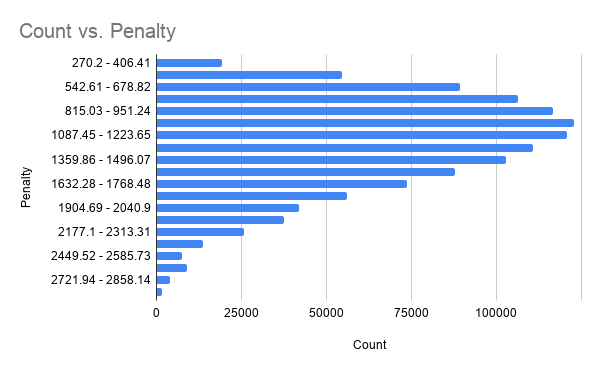
\includegraphics[width=0.65\linewidth]{figs/Count vs. Penalty.png}
    \caption{Distribution of all possible schedule scores}
    \label{fig:score_distribution}
\end{figure}

Additionally, in Table \ref{tab:brute_force_summary} brute forcing took about 3477.30ms. While this is acceptable, if the Unconference were any larger the amount of time needed to brute force would quickly become unreasonable. This is due to the search space growing at a factorial rate in relation to the number of rooms, sessions, and timeslots. However, a heuristic-based approach can be used to obtain good results without needing to search the entire space.

\section{Scheduler Results}
The scheduler was run 100 times using the same data in Table \ref{tab:session_data} to evaluate the quality and consistency of its results. In contrast to brute force search, the scheduler does not check every possible schedule. It uses local search techniques with randomness in order to find a good schedule without searching the entire search space. The results are summarized in Table \ref{tab:scheduler_results}.

  
\begin{table}[h]
\centering

\begin{tabular}{| l | r |}
\hline
\multicolumn{2}{|l|}{Scheduler Results (100 Iterations)} \\
\hline
Avg Score & 327.24 \\
\hline
Median Score & 325.00 \\
\hline
Min Score & 324.1 \\
\hline
Max Score & 340.60 \\
\hline
Avg Time (ms) & 9 \\
\hline
Min Time (ms) & 8 \\
\hline
Max Time (ms) & 12 \\
\hline

\end{tabular}
\caption{Scheduler performance over 100 iterations}
\label{tab:scheduler_results}
\end{table}

\section{Comparison}
As seen in Table \ref{tab:scheduler_results}, the scheduler produces desirable results in comparison to the distribution of all possible scores. The average, min, and max scores are all within the very top portion of the score distribution, meaning all scheduler iterations had scores that were close to optimal. Notably, even the worst schedule the scheduler produced across 100 iterations still falls within the top of the distribution of schedules. While the optimal score wasn't found, all iterations had desirable scores that did not deviate much from one another and were significantly better than the average/median score of all the schedules.

Regarding the amount of time the scheduler took to run, Table \ref{tab:scheduler_results} shows that across 100 iterations it took an average of 9ms, and with a range of 8-12ms. In comparison, it took 3,418ms for the brute force search. That means on average the scheduler had a speedup of nearly 380 times. As the problem scales, this speedup ratio also increases. To demonstrate this we can use 9 sessions from Table \ref{tab:session_data} and simulate two additional scenarios: 3 rooms with 2 timeslots and 2 rooms with 3 timeslots. 

\begin{table}[h]
\centering

\begin{tabular}{|l | l | l | l | l|}
\hline
Timeslots and Rooms & Brute Force (ms) & Scheduler (ms) & Schedules & Speedup\\
\hline
2, 3 & 4.22 & 1.55 & 1680 & 2.72\\
\hline
3, 2 & 18.22 & 1.78 & 7560 & 10.24\\
\hline
3, 3 & 3418 & 9 & 1201200 & 379.78\\
\hline

\end{tabular}
\caption{Scheduler and Brute Force Timing Scenarios}
\label{tab:scheduler_and_brute_force_timings}
\end{table}

In Table \ref{tab:scheduler_and_brute_force_timings}, there are some standouts. First, the brute force search is seeing very rapid growth in how long it takes. Similarly, the total number of schedules is seeing this same explosion of growth. Also, it shows for each scheduling scenario the multiplier for how much faster the scheduler is over brute force search. Specifically, as the scale of the schedule grows, the speedup advantage becomes significant. Something that might be surprising to see is that timeslots affect schedule time and difficulty more than rooms. This is due to the scheduler not treating the permutations of sessions within a timeslot as different schedules.

% \begin{figure}[H]
%     \centering
%     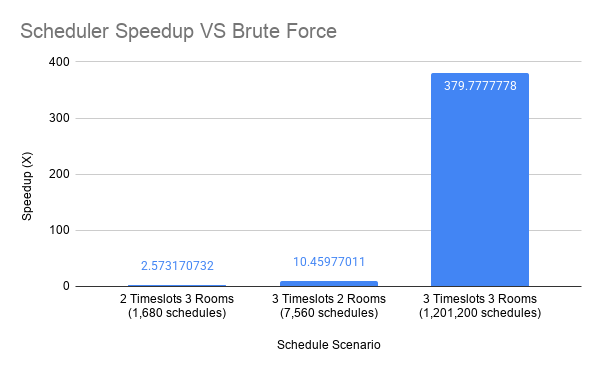
\includegraphics[width=0.75\linewidth]{figs/scheduler_speedup.png}
%     \caption{Scheduler speedup VS brute force search as the scale of the search space grows}
%     \label{fig:scheduler_speedup}
% \end{figure}

While the scheduler did not find the global optimum, it was consistently able to find schedules that were sufficiently close. For Unconference scheduling, the global optimal schedule is not required. An Unconference requires a scheduler that can provide a reasonably good schedule, while being reasonably quick to do so. The scheduler in UnconfRS has demonstrated the ability to find reasonably good schedules in a reasonable amount of time. Additionally, administrators can add schedules manually beforehand. Already determined sessions are not updated by running the scheduler.